\section{私货}
\begin{frame}[fragile]{Typst、M\$ Word 与 \LaTeX{}}
	\begin{itemize}
		\item<+-> Typst:
			\begin{itemize}
				\item Typst很快;支持增量编译;
				\item \LaTeX{}用户惯性大(因为繁杂的缘故);
				\item 可以直接调用 |CSV| 文件——现代生产力水平;
				\item 在据说要打败\LaTeX{}的产品中,生态最好的;
				\item 现代的设计语言风格;
				\item 用比较省力的方式排版出一个基本好看的文档;
				\item 适合不满足于 |Markdown| 功能简陋、又无法接受\LaTeX{}过于冗杂的用户;
				\item 上手容易不代表可以轻松用好它;
				\item 静待期刊支持……
			\end{itemize}
		\item<+-> M\$ Word:
			\begin{itemize}
				\item Word是字处理软件,而不是专门用来排版的;或者反过来,\LaTeX{}不是字处理软件;
				\item 至少上手容易,但同样,不代表可以轻松用好它;
			\end{itemize}
	\end{itemize}
\end{frame}

\begin{frame}{\LaTeX{}3(一)}
	\begin{itemize}
		\item<+-> 为什么要有 \LaTeX{}3?
			\begin{itemize}
				\item \LaTeXe{} 没有很好地实现内容与格式分离的原则;
				\item 因为内核相对较小,当有格式修改需求时,经常遇到功能不足的问题,对格式进行更改需要大量搜索和编写复杂代码;
				\item \CJKsout{就连新定义一些变长参数命令都很麻烦.}
			\end{itemize}
		\item<+-> \LaTeX{}3 旨在——
			\begin{itemize}
				\item 提供现代编程语言的语法与命名规范;
				\item 简化 \LaTeX{} 的宏展开控制;
				\item 标准化 \LaTeX{} 各个功能的接口;
			\end{itemize}
	\end{itemize}
\end{frame}

\begin{frame}[fragile]{\LaTeX{}3(二)}
	\begin{itemize}
		\item (目前的)主要成果 \pkg{expl3} 宏包;
		\item 两个宏包:
		      \begin{itemize}
			      \item 创建用户层命令:\pkg{xparse} 宏包(默认载入);
			      \item 面向对象:\pkg{xtemplate} 宏包
		      \end{itemize}
		\item 一步到位:|texdoc interface3|;
		\item<+-> 懒得学?用 Chat GPT!
	\end{itemize}
\end{frame}

\begin{frame}{得体之术}
	\begin{itemize}
		\item 当甲方的认为比写出良好的代码更紧急的时候……
		\item<+-> \LaTeX{} Hooks!
			\begin{block}{现实案例}
				\begin{center}
					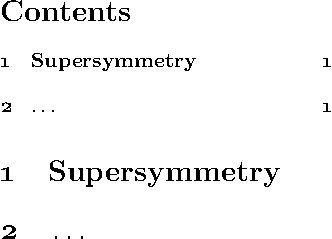
\includegraphics[width = .35\textwidth]{images/Oldtoc.pdf} \kern4\ccwd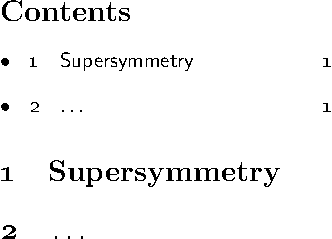
\includegraphics[width = .35\textwidth]{images/Newtoc.pdf}
				\end{center}
			\end{block}
		\item<+-> \pkg{etoolbox} 宏包.偷偷修改(补丁)默认的定义(?).
	\end{itemize}
\end{frame}

\begin{frame}[fragile]{新闻:取所好者}
	\begin{itemize}
		\item<+-> |texdoc ltnews|
		\item<+-> LaTeX Companion 3 发售了;
		\item<+-> \LaTeX{} Hooks.拦截宏展开;
		\item<+-> 整数和浮点数基本计算默认调用: |\inteval|、|\fpeval|;
		\item<+-> 命令和环境复制器.|\NewEnvironmentCopy|(暂未更新)、|\NewCommandCopy|.
	\end{itemize}
\end{frame}

\begin{frame}[fragile]{彩色盒子}
	\begin{tcolorbox}[enhanced,title={\heiti 你想要},frame style image=blueshade.png,colback = 碧蓝!4]
		这样的盒子吗?
		\tcblower
		使用 \pkg{tcolorbox} 宏包!文档:|texdoc tcolorbox|;或者用 |texdoc tcolorbox-example| 查看例子.
	\end{tcolorbox}
\end{frame}

\begin{frame}{文字类排版:字体}
	\begin{itemize}
		\item<+-> 对中文使用者来说,一般使用 \pkg{fontspec} 宏包.
			\begin{itemize}
				\item \CTeX{} 宏集的策略大致是,将 Unicode 字符分成不同的类,每一类单独处理.比如:中文和英文用的就是不一样的字体.
				\item \JPtext{日本語}.当作者意欲在中文内插入日文时,自然应该使用日文字体:
				      \begin{center}
					      八坂神奈子\kern\ccwd 与\kern\ccwd \JPtext{八坂神奈子}
				      \end{center}
				      而不是使用中文字体,这大抵上是最容易出错的细节.
				\item 繁体中文和韩语类似.大陆字体会做日文、韩文部分不代表可以用其来排日文、韩文.
			\end{itemize}
		\item<+-> 如果作者发给你的是 Word 文档,可以先好好沟通一下格式应当如何处理.
	\end{itemize}
\end{frame}

\begin{frame}{文字类排版:OpenType 特性}
	\begin{itemize}[<+->]
		\item 连字:f{}f $\to $ ff, f{}i $\to $ fi, f{}l $\to $ fl;
		\item 老式数字(\texttt{onum}):0123456789 $\to $ {\addfontfeatures{RawFeature={+onum}}0123456789};
		\item 小写大写字母(\texttt{smcp}):An Academic Fantasy For Minority $\to $ {\addfontfeatures{RawFeature={+smcp}}An Academic Fantasy For Minority};
		\item \texttt{case} 特性:{\addfontfeatures{RawFeature={-case}}(西文括号配中文)} $\to $ (西文括号配中文);
		\item 想要知道自己手上字体的 OpenType 特性?\link{https://fontdrop.info}
	\end{itemize}
\end{frame}

\begin{frame}[fragile]{文字类排版:一些碎碎念}
	\begin{itemize}[<+->]
		\item {\bfseries \CJKfontspec[AutoFakeBold = 3]{NotoSerifCJKsc-Medium.otf} 伪粗体}和{\itshape\CJKfontspec[AutoFakeSlant = .16666]{NotoSerifCJKsc-Medium.otf} 伪斜体}.正文中各种意义上都不推荐.但需说明的是,伪斜体可以用在排版代码中的注释.
		\item 罗马数字.{\fontspec{Noto Serif CJK SC Medium}Ⅰ}--{\fontspec{Noto Serif CJK SC Medium}ⅹ},\texttt{U+2160–217F}. Unicode 标准声称收容罗马数字乃是为了兼容性之举,对大多数目的而言应用恰当的拉丁字母列替代之.
		\item 引号.目前常用的蝌蚪形引号有四种(不分中英):
		      \begin{center}
			      \begin{tblr}{cccc}
				      \texttt{U+201C}                                     & \texttt{U+201D}                               & \texttt{U+2018}                                     & \texttt{U+2019}                               \\
				      \makebox[.5\ccwd][l]{\ccbox}\makebox[.5\ccwd][r]{“} & \makebox[0pt][l]{\ccbox}\makebox[\ccwd][l]{”} & \makebox[.5\ccwd][l]{\ccbox}\makebox[.5\ccwd][r]{‘} & \makebox[0pt][l]{\ccbox}\makebox[\ccwd][l]{’}
			      \end{tblr}
		      \end{center}
		      对 \LaTeX{} 和 \CTeX{} 来说,输入以上四种会调用中文字体的全宽引号.欲得到调用西文字体的引号请输入 |`| 和 |'|.
		\item 破折号.破折号可以说是最难以处理的标点,目前没有完美的解决方案.\link{https://github.com/CTeX-org/ctex-kit/issues/382}
	\end{itemize}
\end{frame}

\begin{frame}[fragile]{喜欢的宏包}
	\begin{multicols}{3}
		\begin{itemize}
			\item 必备

			      \begin{itemize}
				      \item \pkg{amsmath}
				      \item \pkg{graphicx}
				      \item \pkg{hyperref}
			      \end{itemize}
			\item 样式

			      \begin{itemize}
				      \item \pkg{caption}
				      \item \pkg{enumitem}
				      \item \pkg{fancyhdr}
				      \item \pkg{geometry}
			      \end{itemize}
			\item 数学

			      \begin{itemize}
				      \item \pkg{bm}
				      \item \pkg{mathtools}
				      \item \pkg{physics2}
				      \item \pkg{unicode-math}
			      \end{itemize}
			\item 表格

			      \begin{itemize}
				      \item \pkg{array}
				      \item \pkg{booktabs}
				      \item \pkg{longtable}
				      \item \pkg{tabularx}
				      \item \pkg{tabularray}
			      \end{itemize}
			\item 插图、绘图

			      \begin{itemize}
				      \item \pkg{subfig}
				      \item \pkg{tikz}
				      \item \pkg{pgfplots}
			      \end{itemize}
			\item 字体

			      \begin{itemize}
				      \item \pkg{newtx}
				      \item \pkg{newpx}
				      \item \pkg{pifont}
				      \item \pkg{fontspec}
			      \end{itemize}
			\item 杂项功能

			      \begin{itemize}
				      \item \pkg{beamer}
				      \item \pkg{biblatex}
				      \item \pkg{fancyhdr}
				      \item \pkg{listings}
				      \item \pkg{mhchem}
				      \item \pkg{siunitx}
				      \item \pkg{xcolor}
			      \end{itemize}
		\end{itemize}
	\end{multicols}
\end{frame}